\begin{figure}[h]
\centering
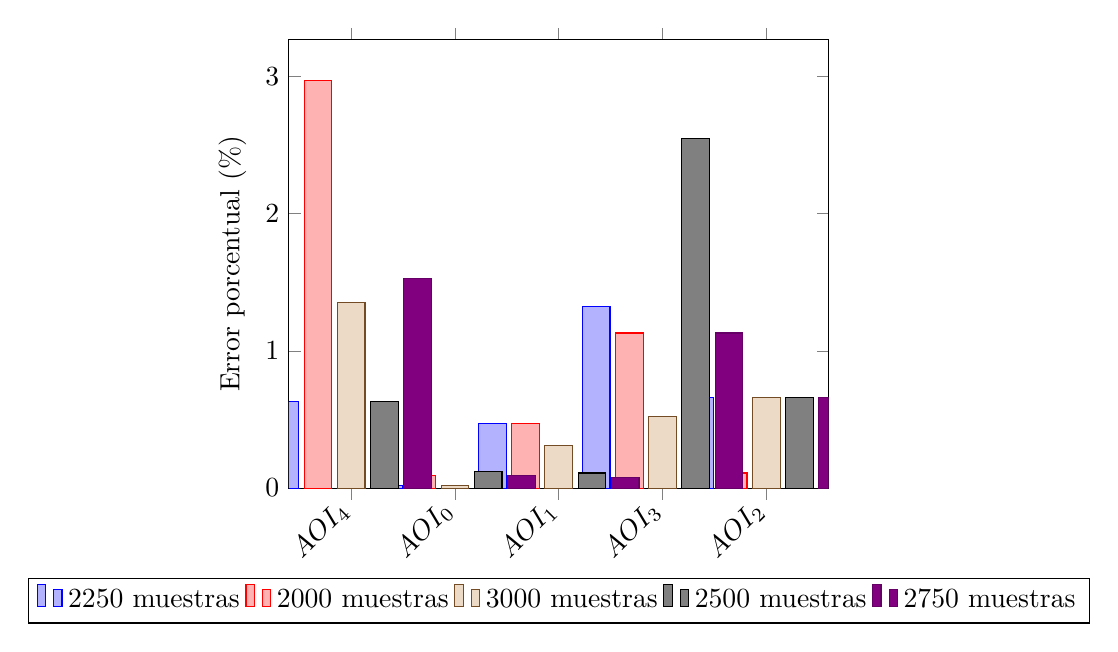
\begin{tikzpicture}
\begin{axis}[
    ybar,
    bar width=10pt,
    ylabel={Error porcentual (\%)},
    xlabel={Áreas de Interés},
    symbolic x coords={$AOI_{4}$, $AOI_{0}$, $AOI_{1}$, $AOI_{3}$, $AOI_{2}$},
    xtick=data,
    x tick label style={rotate=45, anchor=east},
    ymin=0,
    enlarge x limits=0.15,
    legend style={at={(0.5,-0.2)}, anchor=north,legend columns=-1},
    legend cell align={left}
]
\addplot coordinates {
($AOI_{4}$, 0.63)
($AOI_{0}$, 0.02)
($AOI_{1}$, 0.47)
($AOI_{3}$, 1.32)
($AOI_{2}$, 0.66)
};
\addplot coordinates {
($AOI_{4}$, 2.97)
($AOI_{0}$, 0.09)
($AOI_{1}$, 0.47)
($AOI_{3}$, 1.13)
($AOI_{2}$, 0.11)
};
\addplot coordinates {
($AOI_{4}$, 1.35)
($AOI_{0}$, 0.02)
($AOI_{1}$, 0.31)
($AOI_{3}$, 0.52)
($AOI_{2}$, 0.66)
};
\addplot coordinates {
($AOI_{4}$, 0.63)
($AOI_{0}$, 0.12)
($AOI_{1}$, 0.11)
($AOI_{3}$, 2.55)
($AOI_{2}$, 0.66)
};
\addplot coordinates {
($AOI_{4}$, 1.53)
($AOI_{0}$, 0.09)
($AOI_{1}$, 0.08)
($AOI_{3}$, 1.13)
($AOI_{2}$, 0.66)
};
\legend{2250 muestras, 2000 muestras, 3000 muestras, 2500 muestras, 2750 muestras}
\end{axis}
\end{tikzpicture}
\caption{Errores porcentuales por AOI en distintos tamaños de dataset}
\end{figure}